\documentclass[11pt, a4paper, twoside, openright, openany]{article}

\usepackage{graphicx,color}
\usepackage{amssymb, amsmath, array}
\usepackage{cite}
\usepackage[T1]{fontenc}

\usepackage{listings}
\usepackage{color}
\usepackage{dirtytalk}
\usepackage{url}

\graphicspath{{illustrations/}}
\setlength{\parindent}{0pt}
\setlength{\parskip}{\baselineskip}
\begin{document}

\begin{center}
% Example of title page for the projects carried out within DEDIS
% Copied from lasec

% Simply include it in your mastex tex file:
%        % Example of title page for the projects carried out within DEDIS
% Copied from lasec

% Simply include it in your mastex tex file:
%        % Example of title page for the projects carried out within DEDIS
% Copied from lasec

% Simply include it in your mastex tex file:
%        \input{cover}


% Updated October 2016


\newcommand{\logoepfl}[0]{
  \begin{center}
    
\includegraphics[width=4cm]{logo_epfl_coul.eps}
  \end{center}
  \vspace{0.3cm}
  \hrule
}
\newcommand{\project}[1]{
  \begin{center}
    \large{#1}
  \end{center}
  \vspace{1cm}
}
\newcommand{\department}[1]{
  \begin{center}
    \large{#1}
  \end{center}
}
\newcommand{\lab}[1]{
  \begin{center}
    \large{#1}
  \end{center}
}
\newcommand{\supervisor}[3]{
  \begin{center}
    \begin{normalsize}{
        \bf #1}\\#2\\#3
    \end{normalsize}
  \end{center}
}
\renewcommand{\author}[1]{
  \begin{center}
    \Large{#1}
  \end{center}
  \vspace{0.5cm}
}
\renewcommand{\title}[1]{
  \vspace{3cm}
  \begin{center}
    \huge{#1}
  \end{center}
  \vspace{1.7cm}
}
\renewcommand{\date}[2]{
  \begin{center}
    \normalsize{#1 #2}
  \end{center}
  \vspace{0.5cm}
}


\thispagestyle{empty}


% begin title page
  \logoepfl
  
  \title{Web-Frontend for Cothority}

  \author{Bastian Nanchen}
  \department{School of Computer and Communication Sciences}
  \lab{Decentralized and Distributed Systems lab}
  \project{Semester Project}

  \date{December}{2016}

  \begin{center}
    \begin{tabular}{cc}
      \begin{tabular}{p{4.0cm}}
        \supervisor{Responsible}{Prof.Bryan Ford}{EPFL / DEDIS}
      \end{tabular}&
      \begin{tabular}{p{4.0cm}}
        \supervisor{Supervisor}{Linus Gasser}{EPFL / DEDIS}
      \end{tabular}
    \end{tabular}
  \end{center}

% end title page



% Updated October 2016


\newcommand{\logoepfl}[0]{
  \begin{center}
    
\includegraphics[width=4cm]{logo_epfl_coul.eps}
  \end{center}
  \vspace{0.3cm}
  \hrule
}
\newcommand{\project}[1]{
  \begin{center}
    \large{#1}
  \end{center}
  \vspace{1cm}
}
\newcommand{\department}[1]{
  \begin{center}
    \large{#1}
  \end{center}
}
\newcommand{\lab}[1]{
  \begin{center}
    \large{#1}
  \end{center}
}
\newcommand{\supervisor}[3]{
  \begin{center}
    \begin{normalsize}{
        \bf #1}\\#2\\#3
    \end{normalsize}
  \end{center}
}
\renewcommand{\author}[1]{
  \begin{center}
    \Large{#1}
  \end{center}
  \vspace{0.5cm}
}
\renewcommand{\title}[1]{
  \vspace{3cm}
  \begin{center}
    \huge{#1}
  \end{center}
  \vspace{1.7cm}
}
\renewcommand{\date}[2]{
  \begin{center}
    \normalsize{#1 #2}
  \end{center}
  \vspace{0.5cm}
}


\thispagestyle{empty}


% begin title page
  \logoepfl
  
  \title{Web-Frontend for Cothority}

  \author{Bastian Nanchen}
  \department{School of Computer and Communication Sciences}
  \lab{Decentralized and Distributed Systems lab}
  \project{Semester Project}

  \date{December}{2016}

  \begin{center}
    \begin{tabular}{cc}
      \begin{tabular}{p{4.0cm}}
        \supervisor{Responsible}{Prof.Bryan Ford}{EPFL / DEDIS}
      \end{tabular}&
      \begin{tabular}{p{4.0cm}}
        \supervisor{Supervisor}{Linus Gasser}{EPFL / DEDIS}
      \end{tabular}
    \end{tabular}
  \end{center}

% end title page



% Updated October 2016


\newcommand{\logoepfl}[0]{
  \begin{center}
    
\includegraphics[width=4cm]{logo_epfl_coul.eps}
  \end{center}
  \vspace{0.3cm}
  \hrule
}
\newcommand{\project}[1]{
  \begin{center}
    \large{#1}
  \end{center}
  \vspace{1cm}
}
\newcommand{\department}[1]{
  \begin{center}
    \large{#1}
  \end{center}
}
\newcommand{\lab}[1]{
  \begin{center}
    \large{#1}
  \end{center}
}
\newcommand{\supervisor}[3]{
  \begin{center}
    \begin{normalsize}{
        \bf #1}\\#2\\#3
    \end{normalsize}
  \end{center}
}
\renewcommand{\author}[1]{
  \begin{center}
    \Large{#1}
  \end{center}
  \vspace{0.5cm}
}
\renewcommand{\title}[1]{
  \vspace{3cm}
  \begin{center}
    \huge{#1}
  \end{center}
  \vspace{1.7cm}
}
\renewcommand{\date}[2]{
  \begin{center}
    \normalsize{#1 #2}
  \end{center}
  \vspace{0.5cm}
}


\thispagestyle{empty}


% begin title page
  \logoepfl
  
  \title{Web-Frontend for Cothority}

  \author{Bastian Nanchen}
  \department{School of Computer and Communication Sciences}
  \lab{Decentralized and Distributed Systems lab}
  \project{Semester Project}

  \date{December}{2016}

  \begin{center}
    \begin{tabular}{cc}
      \begin{tabular}{p{4.0cm}}
        \supervisor{Responsible}{Prof.Bryan Ford}{EPFL / DEDIS}
      \end{tabular}&
      \begin{tabular}{p{4.0cm}}
        \supervisor{Supervisor}{Linus Gasser}{EPFL / DEDIS}
      \end{tabular}
    \end{tabular}
  \end{center}

% end title page

\end{center}

\tableofcontents

\clearpage

\section{Introduction}
The decentralized and distributed systems (DEDIS) team at EPFL is working among others on a software project called Collective Authority (Cothority).
Cothority is composed of multiple conodes, which are servers running protocols and services.
It implements different applications as Collective Signing (CoSi), Cisc (a distributed key/value storage handled by a blockchain with an SSH-plugin),
Proof of Personhood (prove the existence of humain-being), Guard (use distributed servers to hash passwords),
Status (returns the status of a conode)~\cite{cothorityWiki}.
\newline \newline
Distributed cryptography spreads the operation of a cryptosystem among a group
of servers in a fault-tolerant way~\cite{definition}.
Cothority (Decentralized Withness Cosigning) is a \say{multi-party cryptographic signatures}~\cite{cothorityInfo}.
\newline
In order to accomplish that they developed the CoSi protocol,
which will produce a collective signature by decentralized servers.
To perform a collective signature the protocol needs the hash of a file.
The outcoming signature has the same verification cost and size as an individual signature.
A digital signature is used to verify a file's origin and content.
\newline
This endeavor addresses a significant issue. For example a certificate or a software
update now needs one single signature from a corporation or a government (or anything/anybody) to validate it.
This represents a high-value item for criminals, intelligence agency,\ldots
\newline
The CoSi protocol provides a validation, which is produced by a group of independent parties (named conodes),
at every authoritative statement before any device or client uses it~\cite{cosi}.
\newline \newline
This report initially describes the aims and goals of the semester project.
Then it introduces the tools used for its implementation.
Afterward it describes the problems, that arose during the development of the project
and the solutions found to solve them.
This leads the report to present the results of the project and the theorical and practical limitations of it.
Therefore the report suggests possible future works to improve the project.
At the end the theoritical and practical knowledge gained through the project are depicted and
a step-by-step guide for installation and running of the final product is detailled.
\bigbreak
\section{Aims and goals}
The goal of this semester project is to furnish a web-interface to the Cothority project.
As Cothority's applications, the website uses CoSi and Status.
\newline
The aims stated are to provide a status-table with informations like port number,
name or bandwidth used for each contacted conode, to be able to submit a file for
a digital signature using the CoSi protocol and to verify if a digital signature
corresponds to a particular file.
\bigbreak

\section{Tools used}
Obviously the language choosen to implement the web-interface is JavaScript.
The HTML markup language and the CSS style sheet language are used as well.
\newline
The Bootstrap framework~\cite{bootstrap} is employed for designing the website.
\break

\subsection{Libraries}
Several libraries are used in the semester project.
\newline
The jQuery library~\cite{query} is used to
facilitate the selection and modification of DOM (Document Object Model) elements.
\newline \newline
The protobuf.js~\cite{protobufjs} is a pure JavaScript implementation of Google's Protobuf.
It uses the same format of .proto file.
The Cothority uses Google's Protobuf.
It seems evident to use the same way for the web-interface.
\newline
\say{Protocol buffers are a flexible, efficient, automated mechanism for
serializing structured data-think XML, but smaller, faster, and simpler.}~\cite{protobufDefi}.
\bigbreak

\begin{lstlisting}[caption={Example of .proto file}, captionpos=b]
 message Foo{
            required bytes a = 1;
            optional bytes b = 2;
        }
\end{lstlisting}

A .proto file is composed of protocol buffer message(s). Each message contains name-value pair(s).
The value is a unique tag. Each tag is \say{used to identify your
 fields in the message binary format}~\cite{protobufDefi}.
Each pair has a type. There are multiple disponible tags.
\newline
The last element to define is the rule field. The web-interface
uses two rule fields: \say{required} and \say{optional}. The protocol buffer message
with a \say{required} field is obligate to send or receive the field, contrary to
the message with a \say{optional} field, which is not obligate to send or receive the field in question.
\newline \newline
The js-nacl~\cite{jsnacl} library is adopted in the Verification part of the project.
As said on the library's GitHub page: \say{A high-level Javascript API wrapping an Emscripten-compiled libsodium, a cryptographic library based on NaCl. Includes both in-browser and node.js support.}.
NaCl (Networking and Cryptography library) is a software library written in C for
network communication, encryption, decryption, signatures,\ldots~\cite{nacl}. Its
goal is to \say{provide all of the core operations needed to build higher-level cryptographic tools}~\cite{nacl}.
Little disclaimer NaCl is pronounced \say{salt}.
\newline \newline
Another JavaScript NaCl library TweetNaCl.js~\cite{tweetNacl} is used because
the js-nacl doesn't implement two essential functions.
More will be told when the time comes.
\bigbreak

Other libraries like js-nacl, protobuf.js,etc.\ are used and will be presented
in subsections below.
\bigbreak

\section{Problems that arose and their solutions}
In the following subsections the problems arose and their solutions are treated.
\newline
First the issue of the communication between the client and the server is depicted.
Issue which will lead to the complication generated by asynchronization and how using JavaScript Promise APIs
and generator function the program solves it.
\newline
Afterwards the approach used to send a file for collective signing and the verification of a signature
is detailled.
\bigbreak

\subsection{Communication client/server}
The first problem to tackle was to create a communication between the website
and a conode.
\newline
The object Websocket~\cite{websocketPage} of the JavaScript Web APIs offers the tools to create a communication
between a browser and a server and send/receive data.
\newline
At first an empty protocol buffer message is sent in a Blob~\cite{blob} object containing
the .proto file in bytes.
\bigbreak

\begin{lstlisting}[caption={Empty protocol buffer message}, captionpos=b]
  message Request {
  }
\end{lstlisting}

The request being sent, through a Websocket object, the web page waits for response from the conode.
\bigbreak

\begin{lstlisting}[caption={Response protocol buffer messages}, captionpos=b]
  message ServerIdentity{
      required bytes public = 1;
      required bytes id = 2;
      required string address = 3;
      required string description = 4;
  }

  message Response {
      map<string, Status> system = 1;
      optional ServerIdentity server = 2;

      message Status {
          map<string, string> field = 1;
    	}
  }
\end{lstlisting}

The response is is a map with field corresponding to another message format, which
is a map of a string with a string. Each key corresponds to an element of the conode's
status (port number, hostname, number of bytes received and sent, number of services,
 connexion type, uptime, name and version) and each field to its value.
\bigbreak

\subsection{Asynchronicity}

Nevertheless the response message is triggered by our opening socket message.
Therefore the response message will be asynchronous.
\newline
To tackle the asynchronous problem, the introduction of the JavaScript Promise object shall be made.
\newline
First it is important to know that JavaScript is single threaded.
It means that if a code snippet is waiting on data, the thread can't preempt
and doesn't execute the remaining part of the program. In that case JavaScript programs
would be very slow and no user-integration while waiting would be possible.
So through the history of the JavaScript language many tools were
created to handle asynchronous part of code. Like callback functions that were widely
used, but widely disliked too. It even has a nickname: \say{Callback Hell}.
\bigbreak

\begin{lstlisting}[caption={Example of Callback Hell with its typical pyramid shape}, captionpos=b]
  fs.readdir(source, function (err, files) {
  if (err) {
    console.log('Error finding files: ' + err)
  } else {
    files.forEach(function (filename, fileIndex) {
      console.log(filename)
      gm(source + filename).size(function (values) {
        // some code
        )
          }
        }
      })
    })
  }
})
\end{lstlisting}

Other libraries (e.g. jQuery) begun implementing promises to help developers overcome the \say{Callback Hell}.
This eventually leads ECMAScript 6 to adopt the Promise API~\cite{promise} natively in JavaScript~\cite{ecmaPromise}.
The object Promise allows to retrieve a value in the \say{future}.
\bigbreak

\begin{lstlisting}[caption={Structure of a Promise}, captionpos=b]
  var promise = new Promise(function(resolve, reject) {
    // asynchronous snippet code
    if (/*everything goes well*/) {
      resolve(/*result of async element*/);
    } else {
      reject(/*result of async part*/);
    }
  });
\end{lstlisting}

A callback function needs to be passed at the Promise's constructor. This function
will have at most two parameters. The resolve function (mandatory) will be called
if everything worked in the asynchronous part, otherwise the reject function (optional)
will be called.
\newline
In the case of this semester project, the resolve function will return the response
protocol buffer message containing all the status data from the conode.
\newline \newline
To deal with the Promise object returned the program will use another feature of ECMAScript 6
called a Generator. It's a new kind of function. It can be paused in the middle and
resumed later. Naturally other parts of the code are running during the pause.
\bigbreak

\begin{lstlisting}[caption={Structure of a generator function}, captionpos=b]
  function* foo() {
    var x = yield 1;
  }
  \end{lstlisting}

The \say{*} marks the function as a generator one.
\newline
The other different element, with a traditional function, of the code snippet is the keyword: \say{yield}.
\say{The yield \underline{\hspace{1cm}} is called a \say{yield expression} (and not a statement)
because when we restart the generator, we will send a value back in, and whatever
we send in will be the computed result of that yield \underline{\hspace{1cm}} expression.}~\cite{yieldExpression}.
The function halts when it encounters the \say{yield} keyword.
\newline
Whenever (if ever) the generator is restarted, the \say{yield 1} expression (from the above generator function) will send
\say{1} back. The part following the \say{yield} keyword is the expression that will
be returned.
\bigbreak

\begin{lstlisting}[caption={Restart of a generator function}, captionpos=b]
   var a = foo();
   a.next();
 \end{lstlisting}

The call to the \say{next()} method executes the generator (from the last \say{yield}
until the next encounter of the keyword (if there is any left)).
\newline
Returning to the website's code, a generator function is used with the function returning a Promise object
containing the response protocol buffer message.
\clearpage

\begin{lstlisting}[caption={Extract from the project's code}, captionpos=b]
  function* generator() {
      // some code
      var message = yield websocketStatus("localhost:7003");
      listNodes.push(nodeCreation(message));
      // some code
  }
\end{lstlisting}

The function \say{websocketStatus()} is the one returning the Promise object. The generator function
pauses when reaching \say{websocketStatus()}. \say{The main strength of generators is that they provide a single-threaded, synchronous-looking code style, while allowing you to hide the asynchronicity away as an implementation detail.}~\cite{runGenerator}.
The idea is to \say{yield} out promises and let them restart the generator function when
they are fulfilled.
\newline
To do so we need to create a new function that will control the generator function's iterator.
\bigbreak

\begin{lstlisting}[caption={Extract from the project's code~\cite{runGenerator}}, captionpos=b]
  function runGenerator(g) {
    let iterator = g();
    (function iterate(message) {
      let ret = iterator.next(message);

      if (!ret.done) {
        ret.value.then(iterate);
      }
    })();
  }
\end{lstlisting}

This function takes a generator function as parameter. The \say{iterator} function
variable is the generator function. The inner-function \say{iterate()} looks if
a promise returns the value \say{message} from \say{iterator.next(message)}.
If so, the function waits on it.
\newline
If the generator function is not completed, which implies \say{ret.done} is equal to false, the function will iterate again.

Now all the elements needed, to bring a solution for the asynchronous problem, have
been presented. It only remains to do it for each conode (here in port 7003, 7005, 7009, 7011, 7013).
\clearpage

\begin{lstlisting}[caption={Extract from the project's code reaching some conodes}, captionpos=b]
runGenerator(function* generator() {
  const listAddresses = ["localhost:7003",
      "localhost:7005", "localhost:7007",
      "localhost:7009", "localhost:7011",
      "localhost:7013"];

  window.listNodes = [];
  for (let address of listAddresses) {
        let message = yield websocketStatus(address);
        window.listNodes.push(nodeCreation(message));
  }
  // some code
});
\end{lstlisting}

As said before the \say{websocketStatus()} function returns a Promis object.
Thus the generator function \say{generator()} will halt (\say{yield}) before each
\say{websocketStatus()} call.
\newline
The generator function is given in parameter to the \say{runGenerator()} function.
\newline
The Promise APIs, the generator function and the util function \say{runGenerator()} allow
to hide the asynchronous part of the code. It is more readable and modular.
\bigbreak

\subsection{Collective Signature and Verification}
The following problem to tackle is the implementation of the possibility to send a
file for a collective signature and to verify a signature.
\newline
In the Cothority project the signature is a Schnorr signature, which is a zero-knowledge proof presented
by Mr.Schnorr in 1989. It is \say{based on the intractability of certain discrete logarithm problems}~\cite{wikiSchnorr}.
\newline
In the part where the user can send a file and sign it by the conodes,
the website needs to calculate the aggregate-key using the public-keys of the conodes.
More details will be presented in the Implementation subsection.
\newline
The private and the public-key used in the Cothority project require the usage of
the Edwards-curve Digital Signature Algorithm (edDSA).
\say{edDSA is a variant of Schnorr's signature system with Twisted Edwards curves.}~\cite{edDSA}.
The Cothority project uses Ed25519, which is an instantiation of EdDSA, for the
public-key signature. Ed25519 has some interesting aspect as a fast key generation,
small keys and an high security level~\cite{ed25519}.
\bigbreak

\subsubsection{Send a file for collective signing}
The user has the possibility to submit a file and download a JSON file with the
signature and other informations.

The implementation of the HTML part is straightforward. It uses an input tag to
submit a file and all the collapse-elements are managed by the Bootstrap framework~\cite{bootstrap}.
\bigbreak

\begin{figure}[ht!]
\centering
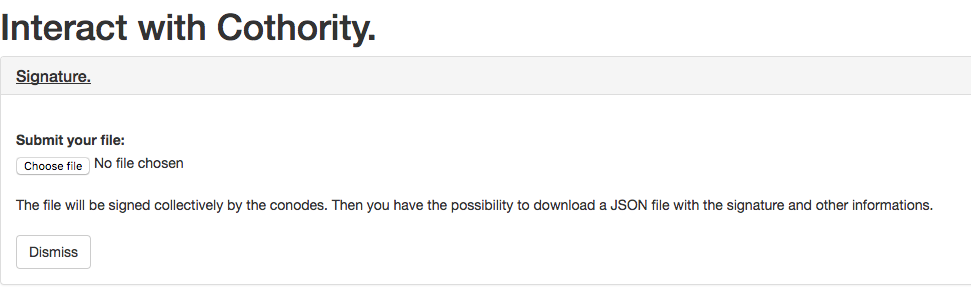
\includegraphics[width=125mm]{verification_signature.jpg}
\caption{Interface}
\end{figure}

The file submitted is read as an ArrayBuffer~\cite{ArrayBuffer}. The Promise APIs,
a generator function and the \say{runGenerator()} function are used to deal with
the asynchronous part of submitting a file. The reading of the file is returned
inside a Promise object in a generator function that is given in paramter to the
\say{runGenerator()} util function (see above for more details on
the manner to tackle the asynchronous part). % TODO come back for the number of the subsection

Afterward the file needs to be signed.

As soon as the websocket is appropriately opened, the communication is done through a websocket
using 4 protocol buffer messages.
\bigbreak

\begin{lstlisting}[caption={.proto file}, captionpos=b]
  message ServerIdentity{
      required bytes public = 1;
      required bytes id = 2;
      required string address = 3;
      required string description = 4;
  }

  message Roster {
      optional bytes id = 1;
      repeated ServerIdentity list = 2;
      optional bytes aggregate = 3;
  }

  message SignatureRequest {
      required bytes message = 1;
      required Roster roster = 2;
  }

  message SignatureResponse {
      required bytes hash = 1;
      required bytes signature = 2;
  }
\end{lstlisting}

For safety reason, the calculation of the aggregate-key shall be done in the program.
The risk is to have a server, which could make up a pair of public and private keys and
then sends the make up public-key to the website as the aggregate-key. The security of
all the servers would be questioning.
\newline \newline
Initially a list of each conode's public-key needs to be created. The status part
of the website looks after collecting servers' informations every 3 seconds. A variable,
which contains all the informations of the conodes, is added to the \say{window} object.
Adding an element to the \say{window} object is a proper way to define a global variable
in JavaScript~\cite{globalVariable}. Thus this list is used to collect each public-key
of the conodes. Having that the calculation of the aggregate-key can begin.
The program utilizes another NaCl library: \say{TweetNaCl.js}~\cite{tweetNacl} to
pack, negatively unpack and addition the points. The function \say{pack()} transforms a point x, y, z, t in Ed25519
into a JavaScript Uin8Array object. On the other hand the function \say{unpackneg()}
transforms a JavaScript Uint8Array object into point x, y, z, t and multiplies
the x-axis by -1. For the reason that it is preferable for operations in the TweetNaCl.js library.
\bigbreak

\begin{lstlisting}[caption={Extract of the code calculating the aggregate-key}, captionpos=b]
const listServers = window.listNodes.map(function(node, index) {
  const server = node.server;
  const pub = new Uint8Array(server.public.toArrayBuffer());
  pub[31] ^= 128;
  const pubPos = [gf(), gf(), gf(), gf()];
  unpackneg(pubPos, pub);
  if (index === 0) {
    agg = pubPos;
  } else {
    add(agg, pubPos);
  }
  // some code
});
pack(aggKey, agg);
\end{lstlisting}

In the above code the variable \say{pub} is the public-key of a conode retrieved thanks to
the global variable \say{window.listNodes}.
\newline
Then the line \say{pub[31] \^{}= 128} is
a multiplication of the x-axis by -1, due to the fact that the TweetNaCl.js has no
an \say{unpack} function but only an \say{unpackneg} function as said before.
\newline
The function \say{gf()} from TweetNacl.js is just a function that returns an array
of \say{0} of size 16. The variable \say{pubPos} is a zero-point.
\newline
Afterward the addition of the point is done using the \say{add()} function from
the TweetNaCl.js library.
\newline \newline
Having calculated the aggregate-key, the website sends to one conode the list of servers
and the hash of the file. On the server side, the server, receiving these informations,
contacts the other conodes to collectively sign the hash of the file using the CoSi protocol.
Then the server responds with a message containing the signature
and the hash of the file. The server's response and the aggregate-key are entrusted to a function
\say{saveToFile(fileSigned, filename, message)}.
\newline
The function takes as parameters the signed file contained inside an ArrayBuffer,
the filename and an array message containing the signature and the aggregate-key.
Then it calculates the SHA-256 hash of the file using a function from js-nacl library.
The signature, the aggregate-key and the hash are translated in base64 for inclusion
as a string in the JSON file.
\newline \newline
From there on the JSON file is created and proposed to be downloaded to the website's user.
The JSON file contains the signature's file, the filename, the date, the aggregate-key and the file's hash.
\bigbreak

\begin{lstlisting}[caption={Example a downloadable JSON file}, captionpos=b]
  "filename": "file",
  "date": "3/12/2016",
  "signature": "vVppwEgya0T22mGlKBfj4Tx+BVQQx0EAH3XFLC
                lfwSbskCxEsPIJ62ZUoD3N7ksRCEK2M/XA6flV
                2tLsiQmrAf4=",
  "aggregate-key": "IjgFxLpeV8IOVShIGC6ESh4cnczF1m5RRS
                    E8jguueG4=",
  "hash": "9UmFDLT4jzzfTMZv/5O71Bh73KTlrOTQXKgKYNC/Z0Y="
\end{lstlisting}

The JSON file is downloadable using a Blob object~\cite{blob}.
\bigbreak

\subsubsection{Verification of the signature}
Having the possibility to sign a file, it seems natural to propose the verification of the latter.
\newline
The user needs to submit a JSON file in the same format as the JSON file downloadable
as previously presented. The website have the ability to perform two verifications.
\newline
First it verifies if the hash of the file is the same as the hash on the JSON file. Second if the signature
is correct knowing the hash and the aggregate-key. The hash is the same as in the first verification
and the aggregate-key is collected from the JSON file.
\newline \newline
The UI section is completed following the same procedure as in the section: \say{Send a file for a collective signature}.
\newline

\begin{figure}[ht!]
\centering
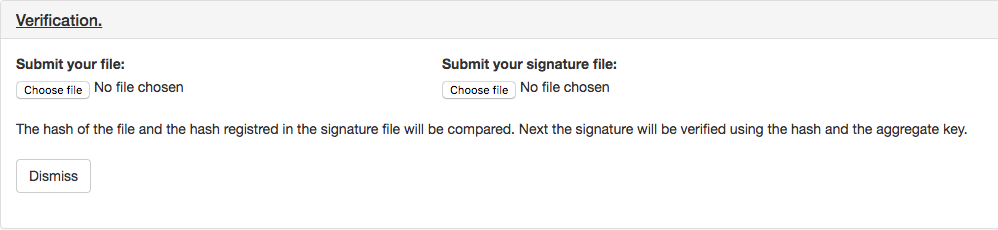
\includegraphics[width=125mm]{verification_verification.jpg}
\caption{Interface}
\end{figure}

The submit of the two files is done in the same way as in the \say{Send a file for a collective signature} part
using Promise APIs, a generator function and \say{runGenerator()} function.
\newline \newline
The program translates the JSON file into an object due to the native function \say{JSON.parse()}.
\newline
It calculates the SHA-256 hash of the submitted file using the same method as in the
section: \say{Send a file for a collective signature} from the js-nacl library.
Next the hash is translated in base64 and the comparison is done character by character.
\newline \newline
The verification of the signature is accomplished using the function
from the js-nacl library \say{nacl.crypto\_sign\_verify\_detached}.
\newline
Careful, the function is experimental but it passed all the tests done during the development.
\newline
The function takes as parameters the signature, the file's hash and the aggregate-key found in
the JSON file. The function returns a boolean depending on the result of the verification.
\newline

\begin{figure}[ht!]
\centering
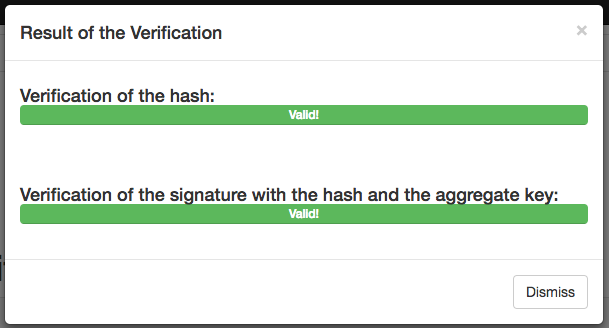
\includegraphics[scale=0.5]{modal.jpg}
\caption{Modal box displaying the result of the verifications}
\end{figure}
%width=125mm
The result of the two verifications is displayed in a modal box.
\bigbreak
\clearpage

\section{Results}
The final product looks like the image below.
\bigbreak

\begin{figure}[ht!]
\centering
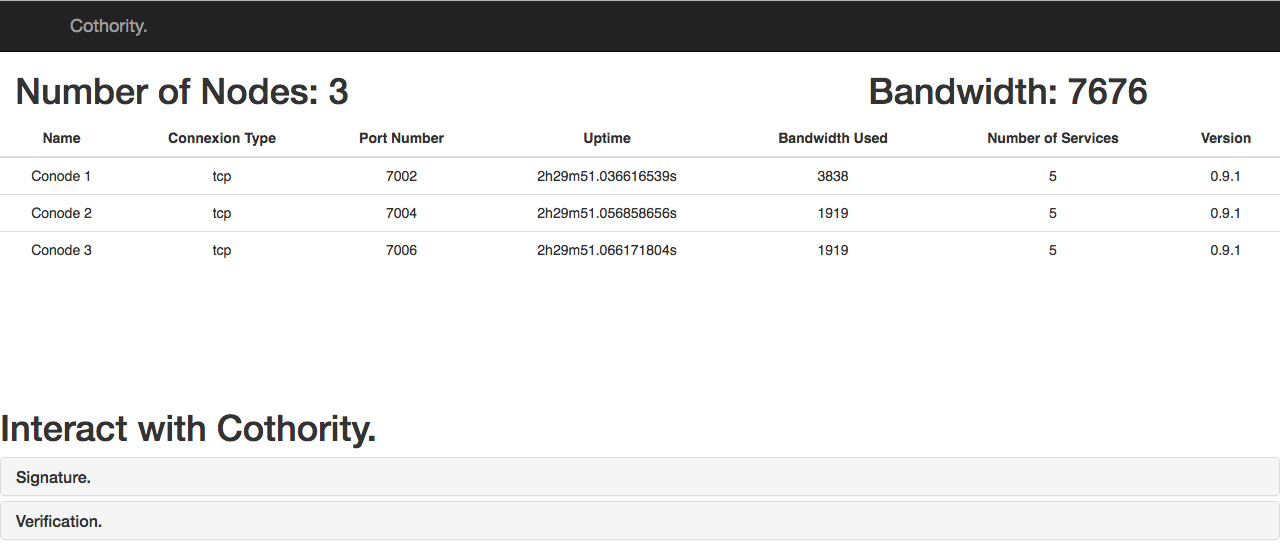
\includegraphics[width=125mm]{interface.jpg}
\caption{Web-interface}
\end{figure}

The status table is refreshed every 3 seconds.
\newline \newline
The website is compatible with Google Chrome and Firefox. It works with Safari
but the browser doesn't let download directly the Blob object on the user's computer. It
opens the Blob object in the browser. The website was not tested on Opera, Microsoft Edge and other web browsers.
\newline \newline
All the libraries are in the project folder. This may seem a bit cumbersome but
it allows more independence and privacy.
\newline

\section{Theoritical and practical limitations of the project}
The website contacts only conodes having their addresses in a static list
(as seen in subsection 4.2 Asynchronicity). It is an inconvenient limitation.
The implementation of the features presented lets no remaining time to tackle
this problem.
\newline
At each instantiation of the js-nacl library, the heap is 32 megabytes in size. Therefore
the user can submit a file of size at most \(\pm\)8.5 megabytes. Certainly this number is
not correct for each computer and each browser but it gives a useful hint.
\newline

\section{Future work}
As written in above section the website contacts only 3 conodes. The next feature
to bring is a recursive function. It will ask each conode to provide a list of each conode
that it knows. Next the program contacts the conodes of the list and so forth.
\newline
It will be necessary to be careful to stop the recursive function at the right time and
to look out conodes that the recursive function as already contacted.
\newline
This new function will also give work on the Cothority project side. When the website
contact a conode it should be able to return the list of known conodes.
\newline \newline
A website is always in development then any new idea can be added.
\bigbreak

\section{Theoritical and practical knowledge gained through the project}
Before this semester project I had never particed HTML, CSS and JavaScript. This
project gave me the opportunity to learn these important languages. The JavaScript language is
one of the most used language at the moment.
\newline
This practical part of web development brought me a theoritical knowledge too.
In how a browser and a website operate. The particularity of single threaded programmation.
\newline \newline
On the cryptographic part, I read some articles on decentralized cryptography.
I understood the importance in the fields of security, integrity and transparency (among others) of decentralized cryptography.
With this semester project in DEDIS laboratory, I was lucky to be able to see it at work through the Cothority project.
\newline
I was able to discover the surface of the elliptic curve signature scheme EdDSA and
one occurence of it: Ed25519, which was useful to tackle the problem of calculating the aggregate-key.
\bigbreak

\section{Step-by-step guide for installation and running of the final product}
\subsection{Installation}
It suffices to open the file \say{cothorityweb.html} in a web browser. The best choice, as
written before, is Google Chrome.
\newline
In the terminal it is important to run a script, which can be found in the folder: cothority/app/cothorityd/
\newline
It is named: \say{run\_cothority.sh}. To run it it suffices to enter: \say{./run\_cothority.sh} in the terminal.
\newline \newline
Then the website comes alive.
\bigbreak

\subsection{Running}
The website is straightforward to use.
\newline

\begin{figure}[ht!]
\centering
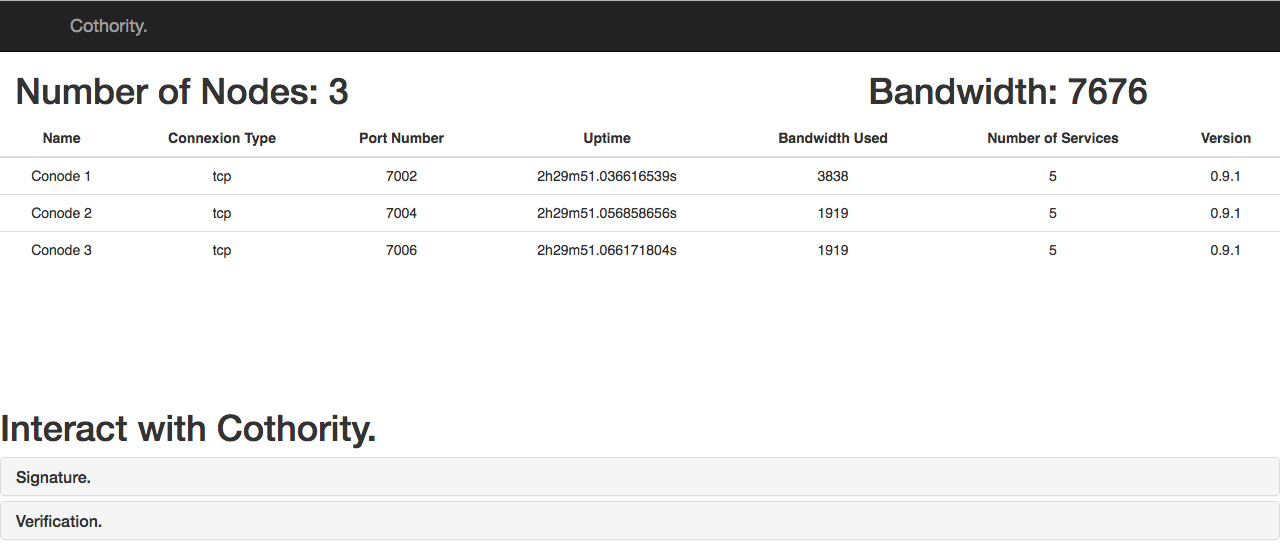
\includegraphics[width=125mm]{interface.jpg}
\caption{Web-interface}
\end{figure}
\leavevmode \newline

The upper part of the web page is dedicated to display the number of conodes, the bandwidth used by all the conodes and
a table containing some information for each conode.
\newline \newline
The bottom part of the web page is consacred to the Signature and Verification parts of the website.
\newline \newline
In clicking on \say{Signature.} a collapse opens and explain how to proceed to sign a certain file.
It only needs to submit a file. After the website has signed it, a download button appears.
It suffices to click on it to load the JSON file, containing the signature, on the computer.
\newline \newline
In clicking on \say{Verification.} a collapse opens and explain how to proceed to verify a signature.
It only needs to submit the file and the JSON file containing the file's signature.
The JSON file must be in the same format as the JSON file downloadable in the Signature part.
\newline
The website displays a monad presenting the result of the verifications. The first if the file's hash and the hash enclosed in the JSON file are the same.
The second if the signature is a correct one knowing the file's hash and the aggregate-key contained in the JSON file.
\bigbreak

\clearpage
\begingroup
\let\cleardoublepage\clearpage
\bibliographystyle{plainurl}
\bibliography{report}
\endgroup

\end{document}
